

(sources will be added later)
This chapter is intended to give the reader an overview of the background knowledge required to understand the rest of the thesis. 
It delves into the foundational concepts of Computer Vision and Deep Learning, elucidating on specific algorithms
and their underlying principles. The importance of reproducibility in scientific research is highlighted, with a particular focus 
on the challenges introduced by randomness in deep learning. This section further dissects the sources of this randomness, 
emphasizing the role of floating-point arithmetic. To provide a practical context, an overview of the datasets, models, and 
the various methods and tools utilized in this research, including optimizers, schedulers, and tracking tools, is presented. 
The aim is to ensure that readers, even those with a peripheral association with the field, can grasp the technical nuances and 
terminologies used throughout the thesis.
\section{Deep Learning}
Deep learning, a salient subset of machine learning, has firmly established itself as one of the pinnacle technological advancements of the modern era. 
This technology, by emulating the structure and functionalities of the human brain through intricate artificial neural networks, enables machines to 
learn and make independent decisions by processing vast data troves.\\

In traditional machine learning, algorithms heavily depended on manual feature extraction. 
This means that before data could be used in a model, its most relevant parts had to be 
pre-identified by humans. In contrast, deep learning models thrive on automation, eliminating 
this manual process. By utilizing multi-layered neural networks, these models intuitively 
identify and extract pivotal features from input data. This unparalleled capability has 
birthed innovations and breakthroughs across numerous domains, from image and speech 
recognition to more sophisticated applications like medical diagnosis and natural language 
processing.\\

The ascendance of automation has only bolstered deep learning's relevance. 
In diverse applications, from robotic processes to customer service automation 
and even the intricate algorithms guiding self-driving vehicles, deep learning 
acts as the backbone. It provides these systems the tools to comprehend their 
environment and subsequently make informed decisions. This integration ensures 
not only unprecedented speed and efficiency but also a level of reliability and 
precision often surpassing human-driven processes.\\

Another frontier that deep learning is significantly influencing is Industry 4.0. 
This term, synonymous with the Fourth Industrial Revolution, marks the ongoing 
transformation characterized by heightened automation and data exchange in manufacturing 
technologies. It encompasses innovations like cyber-physical systems, the ever-expanding 
Internet of Things (IoT), cloud and cognitive computing. Within this ecosystem, deep learning 
emerges as a game-changer. Imagine a manufacturing setup where sensors constantly relay data 
from equipment. Deep learning models, acting on this data, can preemptively detect when a 
component might fail, ensuring timely maintenance, drastically reducing downtime, and 
invariably enhancing production efficiency.\\

To encapsulate, the significance of deep learning in our evolving technological 
landscape is monumental. Whether it's in the seemingly mundane, like fine-tuning 
song or movie recommendations, or in the profoundly impactful, such as diagnosing 
ailments from medical images or forecasting calamities, deep learning stands tall. 
As the world becomes increasingly data-centric, the unparalleled processing and analytical 
capabilities of deep learning models ensure that they remain not just relevant, but 
indispensable. In many ways, deep learning is not merely a trend within artificial 
intelligence; it represents an audacious stride towards devising machines that think and 
learn akin to humans, yet operate on scales unfathomable to human cognition.\\

\subsection{Deep Learning Essentials}

Deep learning, a subset of machine learning, has become a driving force behind various state-of-the-art applications in numerous domains. The following core concepts elucidate the foundational pillars of deep learning, providing insights into its inner workings and methodologies.

\subsubsection*{Neural Networks}

Neural networks are the foundational building blocks of deep learning. They are inspired by the structure and functioning of the human brain's interconnected neurons. The concept of neural networks has gained immense popularity due to their ability to learn complex patterns and representations from data. By simulating the interconnectedness of neurons, neural networks can capture hierarchical features in data, making them suitable for tasks such as image recognition, natural language processing, and more. The layers in a neural network (input, hidden, and output) allow for the extraction of progressively abstract features from the input data, enabling the model to make accurate predictions.
% Insert any specific diagram or visualization you might have for Neural Networks

\subsubsection*{Backpropagation}

Backpropagation is a fundamental algorithm for training neural networks. It is vital because it enables neural networks to learn from data by adjusting their weights and biases. The process involves calculating the gradients of the loss function with respect to each parameter using the chain rule from calculus. These gradients guide the optimization algorithm in adjusting the model's parameters to minimize the prediction error. Backpropagation is crucial for enabling neural networks to learn complex relationships in data, as it iteratively fine-tunes the model's parameters based on the feedback provided by the gradients.
% Insert any specific diagram or visualization you might have for Backpropagation

\subsubsection*{Activation Functions}

Activation functions introduce non-linearity to the neural network, allowing it to approximate and learn complex relationships in data. Without activation functions, neural networks would only be capable of representing linear transformations, severely limiting their expressive power. ReLU, Sigmoid, and Tanh are commonly used activation functions, each with its unique properties. ReLU addresses the vanishing gradient problem, Sigmoid maps inputs to a sigmoid-shaped range suitable for binary classification, and Tanh is often used in hidden layers to map inputs to a range between -1 and 1.
\begin{itemize}
    \item \textbf{ReLU (Rectified Linear Unit):} 
    \[ f(x) = \max(0, x) \]
    
    \item \textbf{Sigmoid:} 
    \[ f(x) = \frac{1}{1 + e^{-x}} \]
    
    \item \textbf{Tanh:} 
    \[ f(x) = \tanh(x) = \frac{2}{1 + e^{-2x}} - 1 \]
\end{itemize}

\begin{figure}[h]
\centering
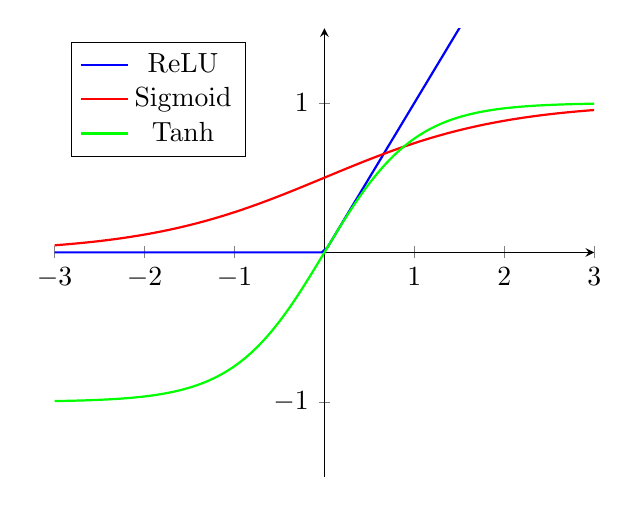
\begin{tikzpicture}
\begin{axis}[
  axis lines=center,
  domain=-3:3,
  ymax=1.5,
  ymin=-1.5,
  samples=100,
  legend pos=north west
]
\addplot[blue, thick] {max(0, x)}; 
\addplot[red, thick] {1/(1 + exp(-x))}; 
\addplot[green, thick] {(2/(1 + exp(-2*x))) - 1};
\legend{ReLU, Sigmoid, Tanh}
\end{axis}
\end{tikzpicture}
\caption{Visualization of Activation Functions}
\end{figure}

\subsubsection*{Loss Functions}

Loss functions quantify the difference between predicted and true values, providing a measure of how well the model is performing. They serve as the basis for optimization, helping the model adjust its parameters to minimize the discrepancy between predictions and ground truth. Different loss functions are used for different tasks; Mean Squared Error (MSE) is well-suited for regression tasks, while Cross-Entropy is commonly used for classification tasks. The choice of the appropriate loss function depends on the nature of the problem the neural network is tackling.
\begin{itemize}
    \item \textbf{Mean Squared Error (MSE)} for regression tasks:
    \[ L(y, \hat{y}) = \frac{1}{n} \sum_{i=1}^{n} (y_i - \hat{y}_i)^2 \]

    \item \textbf{Cross-Entropy} for classification:
    \[ L(y, \hat{y}) = -\sum_{i} y_i \log(\hat{y}_i) \]
\end{itemize}

% You can insert specific diagrams or visualizations for Loss Functions

\subsubsection*{Optimizers}

Optimizers play a crucial role in training neural networks by adjusting the model's parameters to minimize the loss. Gradient Descent and its variants, such as Stochastic Gradient Descent (SGD) and Adam, are essential tools in optimization. These methods determine how the model parameters are updated based on the gradients calculated during backpropagation. Optimizers not only improve training efficiency but also help prevent the model from getting stuck in local minima during optimization.
\begin{itemize}
    \item \textbf{Gradient Descent (GD):} Adjusts each parameter proportionally to the negative of the gradient to find the minimum loss.
    
    \item \textbf{Stochastic Gradient Descent (SGD):} An approximation of GD that computes the gradient using a single training example.
    
    \item \textbf{Adam:} A method that computes adaptive learning rates for each parameter, combining the ideas of Momentum and RMSprop.
    \[ m_t = \beta_1 m_{t-1} + (1-\beta_1)g_t \]
    \[ v_t = \beta_2 v_{t-1} + (1-\beta_2)g_t^2 \]
    Where \( g_t \) is the gradient at time \( t \), and \( m_t \) and \( v_t \) are moving averages.
\end{itemize}

\subsubsection*{Batch Normalization}

Batch Normalization is a technique that improves the training stability and convergence speed of neural networks. It normalizes the intermediate feature representations within a neural network batch-wise. This process helps mitigate the vanishing and exploding gradient problems, enabling smoother and faster convergence during training. Batch Normalization also acts as a regularizer, reducing the need for other regularization techniques like dropout.
\[ \hat{x} = \frac{x - \mu}{\sqrt{\sigma^2 + \epsilon}} \]
Where \( \mu \) is the mean and \( \sigma^2 \) is the variance.

\subsubsection*{Transfer Learning}

Transfer Learning leverages knowledge gained from one task or dataset to improve performance on another related task or dataset. This approach is incredibly useful when labeled data is scarce for the target task. Pre-trained models, especially those trained on massive datasets like ImageNet, provide valuable initializations for the model's parameters. Fine-tuning a pre-trained model on a specific task allows the model to learn task-specific features while retaining the general knowledge it gained from the pre-training.
\subsubsection*{Hyperparameter Tuning}

Hyperparameter Tuning is the process of finding the optimal set of hyperparameters that yield the best performance for a given model and task. Hyperparameters, such as learning rate, batch size, and network architecture, significantly impact the model's training and performance. Efficiently tuning these hyperparameters can lead to faster convergence and better model generalization. Techniques like grid search, random search, and Bayesian optimization help navigate the high-dimensional space of hyperparameters to find optimal combinations.
\subsubsection*{Performance Metrics}

Performance Metrics quantify how well a model is performing on specific tasks. They provide insights into the model's strengths and weaknesses. Accuracy, precision, recall, and F1 score are critical for classification tasks, offering a balanced view of the model's classification abilities. For regression tasks, Mean Absolute Error (MAE) and Mean Squared Error (MSE) measure the deviation between predicted and true values, giving a clear picture of the prediction quality.
\subsubsection*{Data Augmentation}

Data Augmentation is essential for training robust and generalized models, particularly in domains like computer vision. By applying domain-specific transformations to the training data, the model becomes less sensitive to variations in the input data, such as rotation, scaling, and cropping. This technique effectively increases the diversity of the training dataset, helping the model learn more representative features and improving its ability to handle real-world data.
\subsubsection*{Learning Rate Schedulers}

Data Augmentation is essential for training robust and generalized models, particularly in domains like computer vision. By applying domain-specific transformations to the training data, the model becomes less sensitive to variations in the input data, such as rotation, scaling, and cropping. This technique effectively increases the diversity of the training dataset, helping the model learn more representative features and improving its ability to handle real-world data.
\subsubsection*{Early Stopping}

Early Stopping is a regularization technique used to prevent overfitting. Training a model for too many epochs can lead to it memorizing the training data rather than generalizing to new data. Early Stopping monitors the validation performance and halts training when the validation loss starts to increase. This prevents the model from deteriorating on unseen data and helps achieve the best trade-off between training performance and generalization.
% You can insert a visualization here showing training vs validation loss and pointing out where early stopping would intervene.




\subsection{Overview of Deep Learning Algorithms}

Deep learning, over the years, has evolved to cater to diverse domains and challenges, leading to the development of several specialized algorithms. These algorithms emerged in response to specific challenges in data representation, computational efficiency, or domain-specific nuances. The diversity in algorithms is primarily a result of attempts to optimize performance across a myriad of tasks.\\

In chronological order, some of the influential deep learning architectures include Feedforward Neural Networks, Convolutional Neural Networks (CNNs), Recurrent Neural Networks (RNNs), Long Short-Term Memory (LSTM) networks, Gated Recurrent Units (GRUs), and Transformer Networks.

\begin{table}[h]
\centering
\begin{tabularx}{\linewidth}{|l|X|}
\hline
\textbf{Algorithm} & \textbf{Description} \\
\hline
Feedforward Neural Networks & Early architectures designed for pattern recognition without any cycles or loops. \\
\hline
CNNs & Specialized for processing grid-like data, such as images, using convolutional layers. \\
\hline
RNNs & Designed for sequential data, containing loops to maintain information across sequences. \\
\hline
LSTM & An RNN variant addressing vanishing gradient issues and retaining long-term dependencies. \\
\hline
GRUs & Simplified version of LSTMs, offering similar capabilities with fewer parameters. \\
\hline
Transformer Networks & Attention-based models providing parallel processing capabilities and superior performance in sequence tasks. \\
\hline
\end{tabularx}
\caption{Brief overview of key deep learning algorithms.}
\end{table}

\subsubsection*{Convolutional Neural Networks}

CNNs, emerging around the 1980s and popularized in the late 2000s, revolutionized image processing tasks. Unlike traditional Feedforward Neural Networks, CNNs employ convolutional layers, which use filters to scan an input for patterns, significantly reducing the number of parameters and enabling the model to recognize local patterns in data.\\

\textbf{Advantages of CNNs:}
\begin{itemize}
    \item \textit{Parameter Efficiency:} Reduced parameters due to shared weights in convolutional layers.
    \item \textit{Translation Invariance:} Ability to recognize patterns regardless of their position in the input.
    \item \textit{Hierarchical Feature Learning:} Deep architectures extract layered features, moving from basic to complex.
\end{itemize}

% Visualization idea for CNN: A diagram showing how an image is passed through convolutional layers, pooling layers, and fully connected layers.

\subsubsection*{Transformer Networks}

Introduced in the "Attention Is All You Need" paper by Vaswani et al. in 2017, Transformers have since dominated various sequence-based tasks, especially in natural language processing. Instead of relying on recurrence, they use self-attention mechanisms to weigh the importance of different parts of the input data.\\

\textbf{Advantages of Transformer Networks:}
\begin{itemize}
    \item \textit{Parallel Processing:} Lack of recurrence allows simultaneous processing of sequence data, leading to speed gains.
    \item \textit{Long-Distance Dependencies:} Captures relationships in data regardless of the distance between elements.
    \item \textit{Scalability:} Easily scales to handle vast datasets and offers state-of-the-art results in many domains.
\end{itemize}

\textbf{Applications:}
\begin{itemize}
    \item Natural Language Processing tasks like translation, summarization, and question-answering.
    \item Time-series forecasting.
    \item Some computer vision tasks leveraging the Vision Transformer architecture.
\end{itemize}

% Visualization idea for Transformer: A diagram showcasing the self-attention mechanism, highlighting how different parts of an input sequence contribute to the output.
\subsection{Applications of Deep Learning}

Deep learning, an advanced subset of machine learning, has fostered a plethora of innovations across numerous domains due to its unparalleled proficiency in handling vast datasets and extracting intricate patterns. The applicability of deep learning transcends sectors, enabling tasks that were once considered the realm of science fiction.

\begin{itemize}
    \item \textbf{Computer Vision:} From basic image classification to advanced tasks like object detection, segmentation, and facial recognition, deep learning, particularly through Convolutional Neural Networks (CNNs), has redefined the boundaries of what machines can perceive. Autonomous vehicles, medical image analysis, and augmented reality are just a few sectors harnessing the power of deep learning-driven computer vision.
    
    \item \textbf{Natural Language Processing (NLP):} Transformer architectures, most notably the BERT and GPT series, have drastically improved machines' ability to understand and generate human language. This has led to improvements in machine translation, sentiment analysis, and chatbots.
    
    \item \textbf{Speech Recognition:} Voice assistants like Siri, Alexa, and Google Assistant are a testament to the prowess of deep learning in understanding and synthesizing human speech, making voice-activated systems more accurate and ubiquitous.
    
    \item \textbf{Healthcare:} From diagnosing diseases with medical imaging to predicting patient trajectories, deep learning is assisting medical professionals by providing tools that can spot symptoms and patterns often too subtle for the human eye.
    
    \item \textbf{Finance:} In the world of finance, algorithms can predict stock market fluctuations, detect fraudulent activities, and automate trading by leveraging deep learning models.
    
    \item \textbf{Entertainment:} Deep learning-driven recommendation systems, such as those employed by Netflix and Spotify, personalize content suggestions, enhancing user experience. Also, Generative Adversarial Networks (GANs) have been used for art creation, game design, and even music generation.
\end{itemize}

While each of these domains has been transformed by the introduction of deep learning, our primary focus will be on \textbf{Computer Vision}. In the subsequent sections, we will delve deep into its intricacies, methodologies, and advancements, painting a comprehensive picture of how machines `see' and `interpret' visual data.
\section{Computer Vision}

Computer Vision (CV) is an interdisciplinary field that seeks to enable machines to interpret and make decisions based on visual data. Drawing inspirations from human vision, pattern recognition, and computational intelligence, CV has emerged as one of the most significant application areas for deep learning. As \textit{Hubel and Wiesel} pointed out in their groundbreaking studies on the visual cortex \cite{hubel1962receptive}, understanding vision is quintessential to understanding intelligence itself.

\subsection{Image Classification}

At its core, Image Classification is one of the fundamental tasks in computer vision. It involves assigning a predefined label to an input image, usually based on its primary content. For instance, an image containing predominantly a dog would be labeled "dog", irrespective of the breed or its position in the image. In mathematical terms, given an image \(I\), a classifier function \(f\) assigns it a label \(l\) from a set of predetermined labels \(L\):

\[ l = f(I) \]
where \( l \in L \).\\

\textbf{Applications of Image Classification:}
While the rudimentary idea behind image classification might seem simple, its applications have profound impacts on various sectors:

\begin{itemize}
    \item \textit{Medical Imaging:} Diagnosing diseases by classifying medical images into categories like 'tumor' or 'no tumor'.
    \item \textit{Structural Health Monitoring:} Detecting defects or damages in structures like bridges, buildings, and dams by processing and analyzing images or videos. 
    \item \textit{Agriculture:} Identifying unhealthy plants or predicting the type of crops in satellite imagery.
    \item \textit{Security:} Automated surveillance systems detecting unauthorized or suspicious individuals.
    \item \textit{Retail:} Assisting in automated checkout processes by identifying products.
    \item \textit{Automotive:} In autonomous driving, classifying objects helps vehicles make informed decisions, e.g., distinguishing between pedestrians and lampposts.
    \item \textit{Smart Cities:} Analyzing satellite or drone imagery to plan urban development, detect changes in land use, or estimate population densities.
    \item \textit{Finance:} Document classification to identify types of financial statements or bills.
    \item \textit{Social Media:} Content recommendation based on user's photo uploads or identifying inappropriate content.
\end{itemize}

\textbf{Challenges in Image Classification:}

Despite advances, several challenges remain in image classification:

\begin{itemize}
    \item \textit{Intra-class Variation:} Objects of the same class can appear different under varying lighting, angles, or occlusions.
    \item \textit{Scalability:} As the number of categories increases, distinguishing between them becomes harder.
    \item \textit{Data Imbalance:} Some classes might have fewer training samples than others, leading to biased predictions.
    \item \textit{Transferability:} A model trained on one dataset might not perform well on another due to domain shifts.
\end{itemize}


Hubel, D.H., \& Wiesel, T.N.
\textit{Receptive fields, binocular interaction and functional architecture in the cat's visual cortex}.
The Journal of physiology, 1962.

\section{Reproducibility in Scientific Research}

Reproducibility stands as the foundational pillar upon which the edifice of the scientific method has been built. It functions as a rigorous checkpoint, ensuring that scientific findings hold their ground, steadfast and consistent, regardless of who's at the helm of the experiment.\\

In research, methodological variability often emerges as a significant challenge. The slightest nuances in methodology or experimental procedure can drastically alter outcomes. For instance, an experiment conducted at a slightly different temperature or using a subtly different concentration of a reagent can yield results that diverge from the original. As we venture deeper into the realm of research, especially in areas inundated with big data and high-throughput technologies, the challenges multiply. Managing and processing such vast swaths of data in a manner that ensures reproducibility is no small feat.\\

Today's research isn't just a matter of test tubes and microscopes; it's intricately intertwined with software. However, as software evolves, updating and morphing over time, it introduces another layer of variability. An older experiment rerun on a newer software version might produce divergent results, muddying the waters of reproducibility. This software dependency, coupled with the prevalent bias towards publishing positive or novel results, creates an environment where a significant portion of research, especially those yielding negative results, remains shrouded in the shadows, never seeing the light of publication.\\

Yet, the implications of irreproducibility stretch far beyond academic circles. The echoes of irreproducible research reverberate through society, leading to wasted resources as other researchers inadvertently venture down paths based on erroneous findings. More critically, in domains like medicine, the stakes are high. Irreproducible research can mislead clinical practices, culminating in incorrect therapeutic strategies that jeopardize patient health.\\\\\\

\subsection{Irreproducibility in Deep Learning}

(Maybe I eloborate more and introduce and explain the sources of randomness explicitly?)\\

Deep within the neural networks of deep learning lies an inherent stochastic nature that brings with it both challenges and opportunities. This randomness, while fundamental to the training processes of deep learning, also introduces a level of unpredictability that can be both a boon and a bane.\\

At the heart of this randomness is the initialization of weights in neural networks. Starting a model's training journey, these weights are often set to random values, acting as the initial step in a long journey towards optimization. Yet, like setting out on a hike from different starting points, these varied initializations can lead the model to different local optima, influencing the final model's performance.\\

Data augmentation, a technique employed to artificially expand training datasets, further introduces variability. By applying transformations like random cropping or rotation, each epoch of training might expose the model to subtle variations of the same data. While this enhances model robustness, it's another source of randomness.\\

Yet, the landscape of randomness in deep learning isn't just about data and weights. Algorithms like Stochastic Gradient Descent (SGD) introduce their own flavor of unpredictability. By using a random subset of data for weight updates, SGD ensures that the model doesn't just memorize data but learns the underlying patterns. However, this very strength is also a source of variability.\\

Beyond these, computational intricacies, such as floating-point precision in digital computations, especially on GPUs, add their own minute variations. Over millions of operations, these tiny discrepancies accumulate, causing significant variability in outcomes.\\

The randomness issue in deep learning is being actively researched. 
Several studies have approached the issue from various angles. 
For instance, Gundersen et al.~\cite{gundersen2022sources} (fixed later), identified the sources of irreproducibility. 
They found that non-technical sources, such as the initial conditions and the environment of the experiments, affect reproducibility. 
These causes are often related to the mindset and the thinking of the researchers as well as financial constraints. Fig \ref{fig:sources} shows
the non-technical factors that make harder to reproduce any scientific results. These factors indeed valid for deep learning tasks.
Detailed \emph{documentation} with instructions to reproduce to results will help with the reproducibility
and \emph{transparency} on this process would certainly contribute to this cause. Lastly, some \emph{ethics and privacy} regulations could also prevent researchers
to reveal sensitive information, especially in medical domain.
\\
\\

We examine the randomness in this master thesis, which is a technical factor. There are implementation factors and algorithmic factors. These are generally
related with the tooling and the methodology of the experiments. These factors introduce randomness on different level of deep learning process
as a result, variance in the performance occurs. According to Pham et al.~\cite{pham2020problems}, accuracy of the models varies up to \emph{10.8\%}. They conducted a survey as well and
find out that \emph{83.8\%} of the participants unaware of or unsure about implementation level variance. 
Thus, it is reasonable to approach implementation level randomness interrogatively and investigate some standard processes in DL. 
\begin{figure}[htbp]
    \centerline{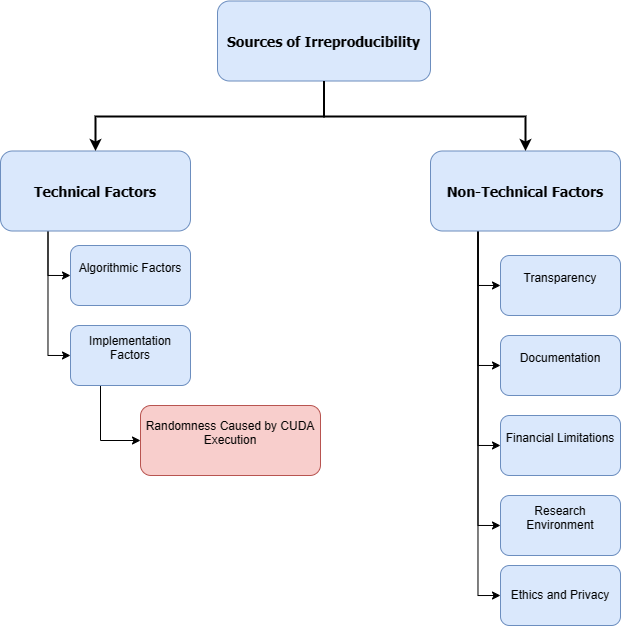
\includegraphics[scale=.5]{Sources.png}}
    \caption{Investigation area of the study.}
    \label{fig:sources}
    \end{figure}
\\
\\
The ripples of this randomness in deep learning extend far and wide. As AI systems become ever more pervasive, from diagnosing diseases to driving cars, unpredictability can pose substantial challenges. Models that yield varying results across runs can complicate evaluations, making direct comparisons challenging. In high-stakes scenarios, like medical diagnoses, this unpredictability can have dire ramifications. Hence, while randomness is an intrinsic aspect of deep learning, understanding, managing, and sometimes mitigating it becomes paramount to harness the true potential of AI.\\
\\

\subsection{Sources of Randomness}
The following presents a full list of algorithmic and implementation factors that introduces randomness~\cite{pham2020problems}~\cite{gundersen2022sources}~\cite{zhuang2022randomness}:
\\
\\
\textbf{Algorithmic Factors}
\begin{itemize}
    \item Nondeterministic DL layers that introduces stochasticity
    \item Random initialization of the weights
    \item Hyperparameter optimization
    \item Data augmentation
    \item Data shuffling and ordering
    \item Batch ordering
\end{itemize}
\textbf{Implementation Factors}
\begin{itemize}
    \item Used framework
    \item Used framework version
    \item Nondeterministic floating point arithmetic
    \item Parallel execution
    \item Auto selection of primitive operations
    \item Unpredictability of processing unit 
\end{itemize}
\subsection{Floating-Point Arithmetics and Parallel Execution}

In the high-performance computing, GPUs have emerged as game-changers. With their vast array of parallel processing units, they have brought unprecedented computational capabilities to the fingertips of developers. NVIDIA's CUDA platform harnesses this power, providing a framework for parallel computing on CUDA-capable GPUs \cite{chetlur2014cudnn}. At the heart of this acceleration lies the intricate dance between floating-point arithmetic and parallel execution.\\

\subsubsection*{Floating-Point Arithmetic: A Double-Edged Sword}

Floating-point arithmetic is the mathematical framework used to represent and operate on real numbers within finite precision. This representation is crucial for many scientific computations, including those in deep learning (DL) networks. However, the limited precision inherent in floating-point arithmetic can introduce errors, and these errors, although typically small, can accumulate over time, especially in iterative algorithms.\\

The IEEE 754 (maybe source needed?) standard defines floating-point arithmetic, ensuring consistency and predictability across platforms. Still, while this standard ensures specific precision levels and behavior for individual operations, it doesn't account for the order of operations. In the realm of parallel computing, where multiple operations can be executed simultaneously or in an unpredictable order, the accumulation and propagation of these errors can introduce non-deterministic behavior.\\

\subsubsection*{Parallel Execution in CUDA: Power and Randomness}

CUDA's parallel execution model divides tasks into threads that are executed across the multiple cores of a GPU. These threads are grouped into blocks, and these blocks are, in turn, organized into grids \cite{chetlur2014cudnn}. This hierarchy allows CUDA to scale computations across different GPU architectures effectively. The figure below illustrates this structure:\\

\begin{figure}[htbp]
\centerline{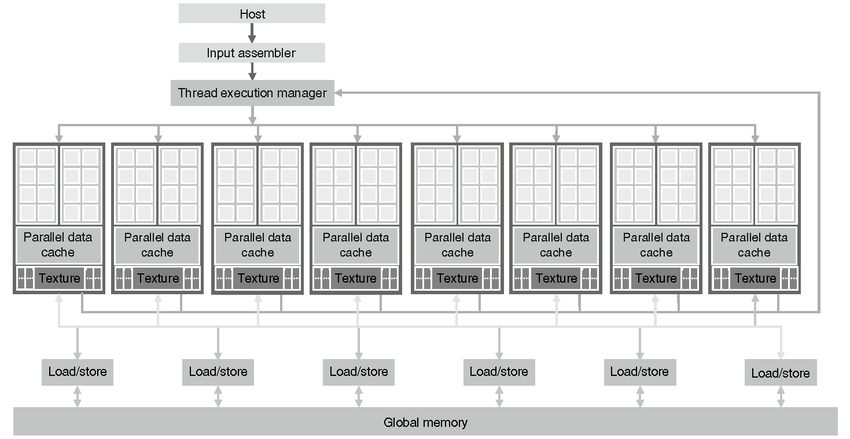
\includegraphics[scale=.8]{cuda.png}}
\caption{Architecture of CUDA-capable GPU. Source:~\cite{chetlur2014cudnn} }
\label{fig:cuda}
\end{figure}

However, the inherent nature of parallel execution introduces randomness due to the unpredictable order in which threads are completed. This randomness is exacerbated when combined with the nuances of floating-point arithmetic. Two runs of the same parallel operation can produce slightly different results due to the varying order of execution and the consequent accumulation of floating-point errors.

\subsubsection*{cuDNN: Leveraging CUDA and Introducing Nondeterminism}

cuDNN is a deep neural network GPU-accelerated library that builds upon CUDA \cite{chetlur2014cudnn}. While it greatly boosts the efficiency of DL networks, some of its operations, such as the CUDA convolution benchmarking, are nondeterministic. This nondeterminism stems from both the scheduling of parallel tasks and the intricacies of floating-point precision. Deterministic execution schemes have been proposed to counteract this issue \cite{chou2020deterministic}. However, these schemes can introduce computational overhead.

\subsubsection*{The Trade-Off: Performance vs. Reproducibility}

There's a delicate balance between performance and reproducibility in parallel computing. Deterministic execution schemes increase the reproducibility and credibility of DL networks, making results more trustworthy and comparable across runs. However, they may come at the cost of increased computational time, which could be a significant drawback in time-sensitive applications or large-scale computations. It is, therefore, essential to analyze and understand these trade-offs carefully, tailoring solutions to specific use-cases and experimental setups.\\

In conclusion, the interplay between floating-point arithmetic and parallel execution in CUDA is a complex one. While it offers immense computational power, it also brings forth challenges in reproducibility. As researchers and developers, it's our responsibility to approach these challenges head-on, understanding their roots and implications, and crafting solutions that balance both performance and reproducibility.

\section{Frameworks and Tools}
The success and efficiency of any scientific study often hinge on the careful selection and proficient use of the right computational tools and frameworks. In the scope of this study, several tools and frameworks have been adopted, each with its unique benefits and contributions to the overall experiment. Here, we provide a brief overview of these tools and their significance in the research.

\subsection{PyTorch}

\textbf{Publisher:} Facebook's AI Research lab (FAIR)\\

\textbf{Overview:}
PyTorch is an open-source deep learning framework that provides a dynamic computational graph, making it particularly suited for research purposes. The framework enables developers to modify the graph on-the-fly, making it versatile and adaptable.\\

\textbf{Role in the Experiment:}
In this study, PyTorch was the primary framework for designing, training, and evaluating deep learning models. Its flexibility allowed for rapid prototyping and experimentation, while its extensive library of functions facilitated the implementation of various network architectures and training methodologies.

\subsection{Weights and Biases (W\&B)}

\textbf{Publisher:} Weights \& Biases, Inc.\\

\textbf{Overview:}
Weights and Biases (W\&B) is a tool designed to help researchers track and visualize experiments in machine learning. It offers capabilities such as hyperparameter tuning, model visualization, and performance tracking, making it a one-stop solution for ML experiment management.\\

\textbf{Role in the Experiment:}
W\&B played a pivotal role in managing the experiments. It was used to log experimental results, visualize model performance over time, and compare different model architectures and hyperparameters. The tool streamlined the experimentation process, ensuring that insights were easily extracted and that optimal model configurations were identified with efficiency.

\subsection{SLURM}

\textbf{Publisher:} SchedMD\\

\textbf{Overview:}
SLURM (Simple Linux Utility for Resource Management) is an open-source job scheduler designed to allocate computational resources in multi-user clusters. It's widely adopted in high-performance computing environments due to its scalability and robustness.\\

\textbf{Role in the Experiment:}
Given the computationally intensive nature of deep learning tasks, SLURM was employed to manage job submissions to a computer cluster. It ensured efficient resource allocation, allowing multiple experiments to be conducted in parallel without resource contention. By queuing and prioritizing tasks, SLURM optimized the utilization of computational resources, ensuring timely execution and completion of experiments.\\

The synergy of these tools and frameworks enabled a seamless, efficient, and insightful experimental process. PyTorch offered the foundational deep learning capabilities; Weights and Biases ensured that experiments were tracked, visualized, and optimized; and SLURM managed the computational resources effectively. Together, they ensured that the research was conducted in a structured, efficient, and reproducible manner.
 
